%This work is licensed under the Creative Commons Attribution-NonCommercial-NoDerivs 3.0 United States License. To view a copy of this license, visit http://creativecommons.org/licenses/by-nc-nd/3.0/us/ or send a letter to Creative Commons, 444 Castro Street, Suite 900, Mountain View, California, 94041, USA.

In Chapters \ref{chap:previous_models} through \ref{chap:model_results}, I have explored the mathematical side of designing an ultrafast electron microscope; modeling the behavior of a pulse and the effect that column elements have upon it.
However, microscopy is an experimental science, and designing a UEM is no less hands-on.

It is our belief that a successful UEM project cannot simply stem from small modifications to the platform of a conventional electron microscope.
In this chapter I describe the prototype UEM system that is being built at UIC.
By necessity much of it is custom built, specifically designed to either allow flexibility or to meet some technical challenge.

\begin{figure}
  \centering
  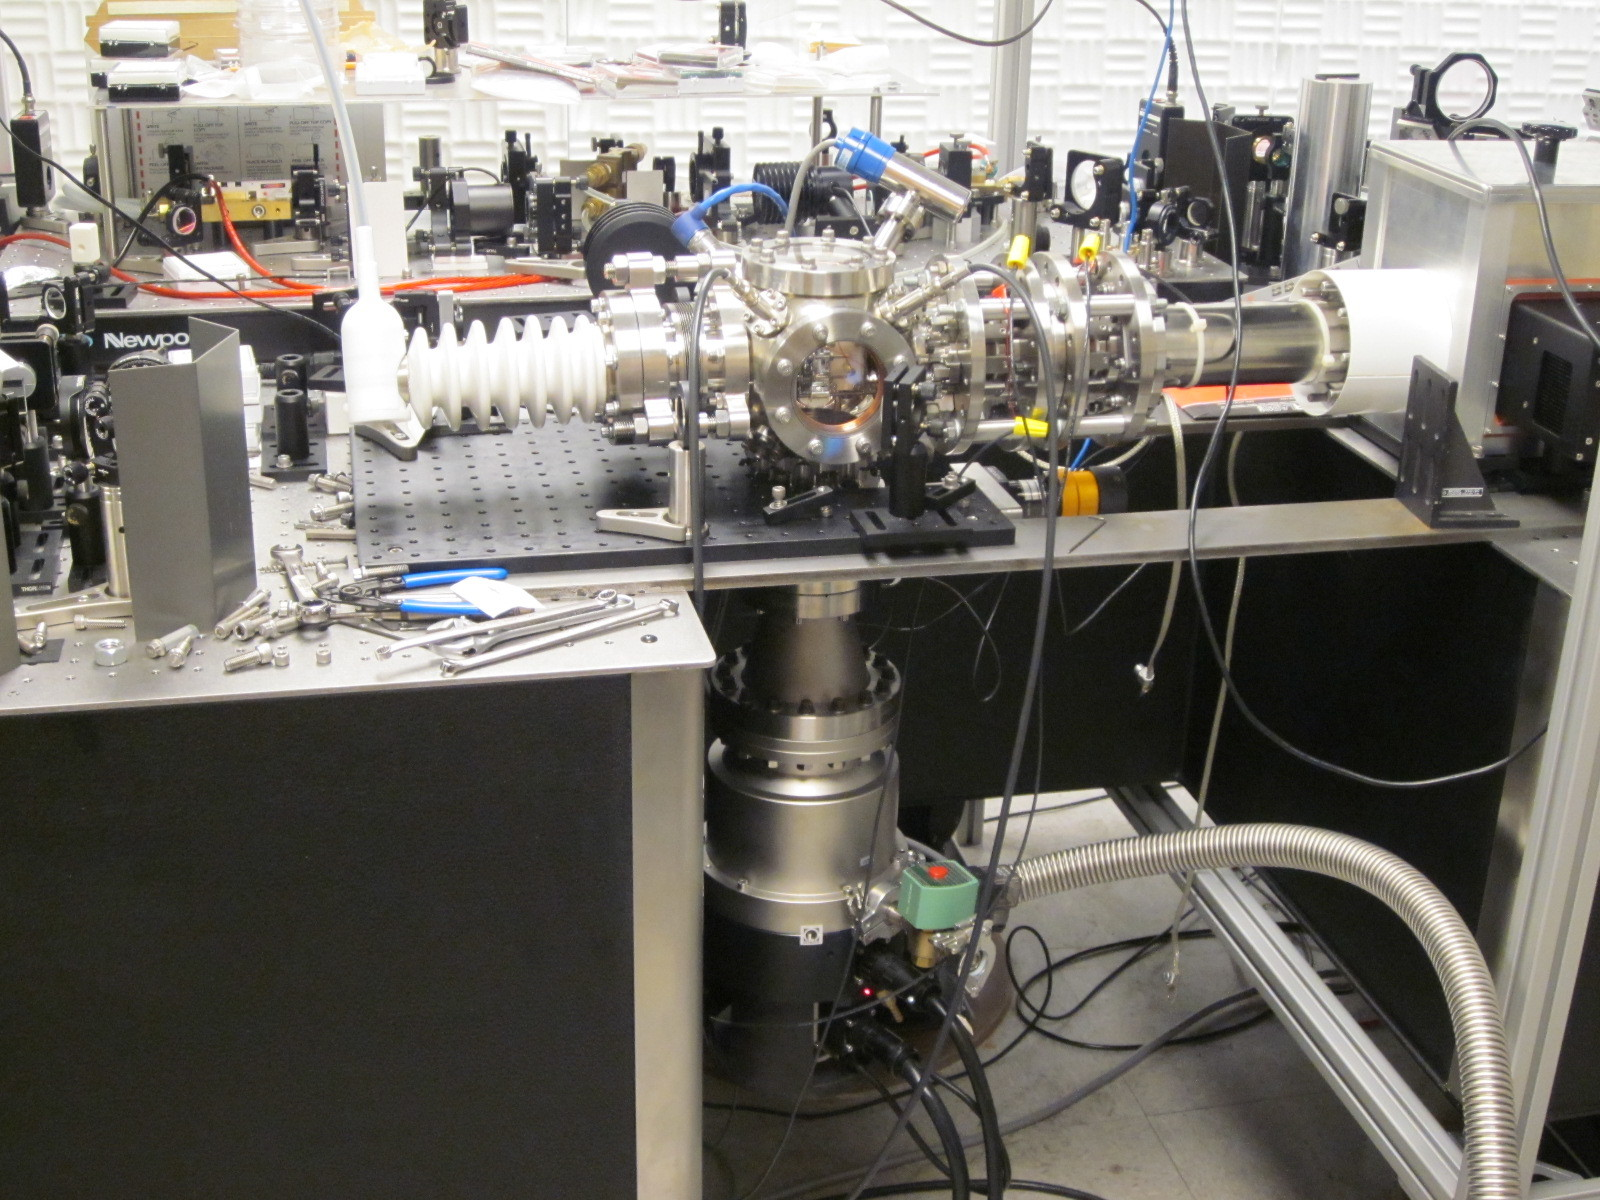
\includegraphics{inc/hardware/column.jpg}
  \caption[Picture of the prototype UEM column at UIC]{
    Picture of the majority of the prototype UEM column at UIC.
    The main vacuum chamber is laid sideways, with the high voltage (gun) at the left and the imaging system on the right.
    The magnetic levitated turbo pump hangs below the column, a scroll pump used for backing is not pictured.
    The laser system is in the background.
    All of the above is mounted on a custom shaped active vibration-canceling optical table.
    The electronic control systems are not pictured.
  }
  \label{fig:column-pic}
\end{figure}


